\documentclass[11pt]{article}

%Erweiterung desr mathematischen Zeichenssatzes
\usepackage{amsmath}
\usepackage{amsfonts}
\usepackage{amssymb}
\usepackage{graphicx}

%Weitere Pakete
\usepackage{makeidx}
\usepackage{framed}
\usepackage{subfig}
\usepackage{amsmath}
\usepackage{hyperref}
\usepackage{caption}
\usepackage{mathdots}
\usepackage{multirow}
\usepackage{underscore}

%Layout
\usepackage[T1]{fontenc}
\usepackage{fancyhdr}
\usepackage[left=4.0cm, right=2.0cm, top=2.00cm, bottom=2.00cm]{geometry}
\usepackage[T1]{fontenc}
\usepackage[bitstream-charter]{mathdesign}
\usepackage[onehalfspacing]{setspace}

% Literaturverzeichnis.
\usepackage[authoryear]{natbib}

% Umbenennungen.
\renewcommand{\refname}{Literaturverzeichnis}
\renewcommand{\figurename}{Fig.}
\renewcommand{\listfigurename}{Abbildungsverzeichnis}

%Benennung
\author{Vorname, Name\\Matrikelnummer: }
\title{\textbf{Implementation of Repeated Measures ANOVA}\\ Statistical Programming Languages \\[5cm]}
\date{\today}
\parindent0pt

% Formartierter Code
\usepackage{listings}
\usepackage{color}

\definecolor{dkgreen}{rgb}{0,0.6,0}
\definecolor{gray}{rgb}{0.5,0.5,0.5}


\lstset{frame=tb,
	language=R,
	aboveskip=3mm,
	belowskip=3mm,
	showstringspaces=false,
	columns=flexible,
	basicstyle={\small\ttfamily},
	numbers=none,
	numberstyle=\tiny\color{gray},
	%keywordstyle=\color{blue},
	commentstyle=\color{dkgreen},
%	stringstyle=\color{mauve},
	breaklines=true,
	breakatwhitespace=true,
	tabsize = 1
}


\pagestyle{fancy}
\fancyhf{}
\rhead{Implementation of Repeated Measures ANOVA}
\lhead{Summes of Suares}
\cfoot{Seite \thepage}

\begin{document}
	\maketitle
	\thispagestyle{fancy}
	\newpage
	\tableofcontents
	\newpage
	\section{Theory and Motivation}
		The main goal of this project is to create an R-package, which bundles a number of functionality around the grand topic of oneway repeated measures Anova (rm ANOVA). Some of the implemented functions are not yet avaiable in R, although the repeated measures anova itself is avaiable. But a functionality to curb with breach of sphericity and correction of confidence intervals are not avaiable.\\
		
		The Ringelmann-effect describes the decreasing individual work performance when work is done in a group. It is therefore often cited in the context of social loafing. The effect was first examined and described by the french agricultural professor Maximillian Ringelmann in his paper from 1913 \citep{ringelmann1913research}. 
	
	\section{Data Simulation}
				 In order to demonstrate and evaluate the functions implemented in the package, we have developed a function to simulate data. It can then be used to test code or for educational purposes. First, we will present the functionalities and the implementation of the simulation function.\\
				 
				 \begin{lstlisting}
				 # Run the data simulation
				 rma_data = sim_rma_data(n = 1000, k = 4, means = NULL, poly_order = 5, noice_sd = c(10, 20, 30, 20), between_subject_sd = 40, NAs = 0)
				 
				 \end{lstlisting}
				 
				 The data can be simulated by running the function shown above, which then returns a dataframe object. The function allows for a number of arguments to be passed. This makes it possible to simulate data with numerous features such as orthogonal polynomial trends and breach of sphericity.\\
				 
				 The first argument \textit{n} is obligatory and defines the number of observation. The argument \textit{k} sets the number of factor levels to be simulated. The output of the function will therefore be an matrix of size $n * (k + 1)$. The first column contains the subject ids to identify each simulated observation and the following columns contain the simulated realization for each factor level.\\
				 
				\begin{lstlisting}
if (!is.null(means)) {
con_means = means
					    
# Check if length of mean vector corresponds to k
if (length(means) != k) {
k = length(means)
print("Number of factors (k) was changed, because the length of means vector and argument k do not correspond.")
}
} else {
			    
# Simulate conditional means
if (is.null(poly_order)) {
con_means = runif(k, min = 100, max = 300)
} else {
					    
# Generate polinomial conditional means
factors = runif((poly_order + 1), min = 0, max = 1)
x = order(runif(k, min = 100, max = 300), decreasing = FALSE)
con_means = matrix(factors[1], nrow = k)
			    
for (p in (2:(poly_order + 1))) {
con_means = con_means + factors[p] * x^p
}
}
}
				\end{lstlisting}
				 
				 The first step, when simulating the data, is to simulate the mean of each factor level. Thereby, each factor level column is filled with the mean for the corresponding factor level. This results in all observations having the same value for each factor level. Additionally, by passing an integer not larger than \textit{k} to the argument \textit{poly\_order}, the means will be simulated so that they create a polynomial trend in the data. Instead of passing an integer \textit{k}, a vector with \textit{k} means can be passed to the argument \textit{means}. This makes it possible to create data with a custom relationship between the factor levels.\\
				 
				 The next step is to simulate the between subject variance and add the subject means, so variation is created between each subject. This is accomplished by adding a matrix of the size \textit{n x k} with normal distributed random numbers to the realizations. The standard deviation of the normal distribution from which the subject deviations are drawn can be controlled with the argument\textit{between\_subject\_sd}. \\
				 
				 The last step  of the simulation is to add noise to the simulated data. The size of the noise can be controlled by passing an integer to the argument noise. It is also possible to pass a vector of length \textit{k}, which makes it possible to simulate data which does not satisfy the sphericity assumption. By simulating different standard deviations for each factor level, the factor level differences also have different variance.
				 
	\section{Data Preparation}
	When computing a Repeated Measures ANOVA, the way to deal with missing values (NAs) is listwise deletion. As we measure the same subjects over different factor levels, a missing value in one factor level leads to a dropout of the whole observation from our analysis.\\
	
	Since we use simulated data, we could easily avoid having missing values. However, for demonstration purposes as well as for applicability to other data, implementing a listwise deletion is necessary. In the above mentioned data simulation function \textit{rma\_data}, the number of NAs is specified, that then randomly replace values of factor levels in the simulated data. Before the data is later processed, in any of the subsequent functions we apply listwise deletion. Hereby, it is checked for existing NAs and the corresponding subject(s) is/are dropped out, while displaying a message informing about the id(s) of the subject(s) that has/have been deleted.\\
	
	\begin{lstlisting}
	# Listwise deletion
	deletionvector = vector(mode = "numeric", length = 0)
	
	for (i in 1:nrow(rma_data)) {
	if (anyNA(rma_data[i, ])) {
	deletionvector = union(deletionvector, i)
	print(paste("Listwise deletion due to missing value(s) for subject", i))
	}
	}
	
	rma_data = rma_data[-deletionvector, ]
	\end{lstlisting}
	
	
	
	
	\section{Repeated Measures ANOVA} 
	Center of our analyses is the Repeated Measures ANOVA model. Since the Repeated Measures ANOVA is a variation of the ANOVA model, we will first give the necessary background information on the ANOVA model. Subsequently, we will present the computation of our Repeated Measures ANOVA model.
	
	\subsection{Based on the ANOVA model}
	The (one-way) ANOVA, an abbreviation for "Analysis of Variance", is used to analyse the dependency between an interval scaled dependent variable and a categorical independent variable. The independent variable must therefore have at least two different categories, which are called factor levels in the ANOVA context. It is then tested, whether differences in the means of the dependent variable broken down by the factor levels of the independent variable can be found. The hypotheses for \textit{k} factor levels are therefore given by:
	
	\begin{eqnarray*}
		H_{0}: {\mu_{1}} = {\mu_{2}} = ... = {\mu_{k}} \\
		H_{1}: \exists i \not= j: {\mu_{i}} \not= {\mu_{j}} 
	\end{eqnarray*} 
	
	The test is accomplished by a decomposition of variance of the dependent variable. From the decomposed elements, the sum of squares of the unrestricted model and the restricted model are computed. In the former, different means for each factor level are assumed, whereas in the latter no such difference is assumed. By use of the F-test, the unrestricted and the restricted model are then compared in order to make a decision on the hypotheses.\\
	
	An important requirement in order to compute an ANOVA are independent data. This requirement is fulfilled, when different subjects are measured in each of the factor levels. Complimentary, in case of dependent data, the Repeated Measures ANOVA is an appropriate model. The Repeated Measures ANOVA is taking use of the dependency structure by additionally calculating the variance between subjects. This subject variance can be separated from the error variance. As a consequence, a high subject variation (with regard to our simulated data: large differences in pulling weights between our subjects) does not lead to a loss of power in the F-test. We will take a closer look at this property of the Repeated Measures ANOVA in section 5.2XXX.
	
	\subsection{Repeated Measures ANOVA Model}
	The computational steps of the Repeated Measures ANOVA implementation will be explained in the following by means of our code. All of these are part of the following function:\\
	
	\begin{lstlisting}
	# Repeated Measures ANOVA function
	rma(rma_data, id = 1)					
	\end{lstlisting}
	
	The first argument specifies the data that is used to compute the Repeated Measures ANOVA. For our purposes, we use our simulated data. The argument \textit{id} specifies the column position of the subject ids. We first define the needed constants and check for the requirements of the data. If any of the requirements is not fulfilled, we stop the computation and display the corresponding requirement in a warning message. Section 7XXX is dealing with error handling in greater detail.\\
	
	\begin{lstlisting}
	# Number of subjects
	n = nrow(rma_data)
	
	# Number of factor levels
	k = ncol(dependent_variable)
	\end{lstlisting}   
	
	In order to compute the Repeated Measures ANOVA, we need to decompose the variance of the dependent variable. For that, we define the basic ANOVA components. Each of the components is given by a matrix of size of the used data \textit{n x k}. The baseline component is hereby just the overall mean of the dependent variable. The factor level component is then given by the difference between the means of the dependent variable conditional to the factors of the independent variable. It has already been mentioned, that, in contrast to the ANOVA model, the variance between subjects is calculated separately for the Repeated Measures ANOVA model. Hence, we specify a subject component, which is given by the difference between the individual means of each subject and the overall mean of the dependent variable. By subtracting the three components from the values of the dependent variable, we then get the error component, containing the individual errors for each subject under each factor level.\\
	
	\begin{lstlisting}  
	# Define basic anova components    
	grand_mean = mean(dependent_variable)
	baseline_components = matrix(grand_mean, nrow = n, ncol = k)
	
	conditional_means = colMeans(dependent_variable)
	factor_level_components = matrix(conditional_means - grand_mean, nrow = n, ncol = k, byrow = TRUE)
	
	subject_means = rowMeans(dependent_variable)
	subject_components = matrix(subject_means - grand_mean, nrow = n, ncol = k)
	
	error_components = dependent_variable - baseline_components - factor_level_components - subject_components
	\end{lstlisting}  
	
	After having computed these basic ANOVA components, we construct the so called decomposition matrix. The decomposition matrix stacks together the vectorized ANOVA components and is used for further computation. Hence, it consists of \textit{k*n} rows and five columns; one column for the original values, one for the baseline component, one for the factor level component, one for the subject component and one for the error component. By squaring each element of the decomposition matrix and summing up the results column-wise, we obtain the sum of squares of each ANOVA component.\\
	
	\begin{lstlisting}      
	# Construct decomposition matrix     
	decomposition_matrix = data.frame(dependent_variable = as.vector(dependent_variable), baseline = as.vector(baseline_components), factor_level = as.vector(factor_level_components), subject_level = as.vector(subject_components), error = as.vector(error_components))
	
	# Compute sums of squares
	ss = as.data.frame(t(colSums(decomposition_matrix^2)))
	rownames(ss) = "sums_of_squares"
	\end{lstlisting}      
	
	Subsequently, we define the degrees of freedom. These are then used to compute the mean squares of the decomposed components. Further we compute the corrected total sum of squares, which can be used to derive the variance in the dependent variable.\\
	
	\begin{lstlisting}
	# Set degrees of freedom
	dof = data.frame(dependent_variable = n * k, baseline = 1, factor_level = k - 1, subject_level = n - 1, error = (n * k) - 1 - (k - 1) - (n - 1))
	
	# Compute mean squares
	ms = ss/dof
	rownames(ms) = "mean_squares"
	
	# Compute corrected total sum of squares
	corrected_sst = ss$dependent_variable - ss$baseline
	variance = corrected_sst/(dof$dependent_variable - dof$baseline)
	\end{lstlisting}   
	
	Having defined all components needed, the F-test and the corresponding p-value are computed.\\
	
	\begin{lstlisting}   
	# Compute F-values 
	F_value_factor = ms$factor_level/ms$error
	F_value_baseline = ms$baseline/ms$subject_level
	
	# Set p-values of F distribution 
	p_factor = 1 - pf(F_value_factor, dof$factor_level, dof$error)
	p_baseline = 1 - pf(F_value_baseline, dof$baseline, dof$subject_level)
	\end{lstlisting}   
	
	Last, we create the output table for the Repeated Measures ANOVA. The table contains the sum of squares, the degrees of freedom, the mean squares, the F-values as well as the p-values for each of the components. By running the funtion \textit{rma}, this output table is always printed. The Repeated Measures ANOVA-table for the simulated data used in our analysis is given by table \ref{table:outputtable1} on page \pageref{table:outputtable1}. It can be seen, that the F-tests are highly significant. The baseline-F-test hereby tests, whether the overall mean is equal to zero, which can be rejected in our case. The Factor-F-test then tests the hypotheses outlined in Section 4.1XXX. Hence, we can reject the $H_{0}$, stating that the factor level means are all equal.\\
	
	\begin{lstlisting}   
	# Create the output table for rmANOVA
	
	# Specify source variable
	source = c("Baseline", "Factor", "Subject", "Error", "Total", "Corrected total")
	
	# Create table
	ANOVA_table = data.frame(check.names = FALSE, Source = source, `Sum of squares` = c(ss %>% select(2:5, 1) %>% unlist(), corrected_sst), `Degrees of freedom` = c(dof %>% select(2:5, 1) %>% unlist(), (n * k) - 1), `Mean squares` = c(ms %>% select(2:5) %>% unlist(), NA, variance), `F-value` = c(F_value_baseline, F_value_factor, NA, NA, NA, NA), `p-value` = c(p_baseline, p_factor, NA, NA, NA, NA))
	
	rownames(ANOVA_table) = NULL
	\end{lstlisting}   
	
	\begin{table}[ht]
		\centering
		\begin{tabular}{rlrrrrr}
			\hline
			& Source & Sum of squares & Degrees of freedom & Mean squares & F-value & p-value \\ 
			\hline
			1 & Baseline & 1769610.20 & 1 & 1769610.20 & 1430.36 & <0.001 \\ 
			2 & Factor & 174706.07 & 4 & 43676.52 & 142.23 & <0.001 \\ 
			3 & Subject & 33403.82 & 27 & 1237.18 &  &  \\ 
			4 & Error & 33166.05 & 108 & 307.09 &  &  \\ 
			5 & Total & 2010886.14 & 140 &  &  &  \\ 
			6 & Corrected total & 241275.94 & 139 & 1735.80 &  &  \\ 
			\hline
		\end{tabular}
		\caption{Repeated Measures ANOVA-table for our simulated data.}\label{table:outputtable1}
	\end{table}
	
	
	
	
	
	
	\section{Reduction of Error Sum of Squares}
	The Repeated Measures ANOVA is closely related to the ANOVA, however used for dependent data. Hence, in the following section, we want to take a closer look at the differences between both models. In order to do so, we compute an ANOVA model and compare its error sum of squares with the ones of the Repeated Measures ANOVA model (section 4.2XXX).	Such comparison is only made for the purpose of demonstrating the model differences. Since ANOVA requires independent data, it would give us misleading results when computed for of our simulated data.\\
	
	
	
	\subsection{Estimation of our ANOVA model}
	In order to enable a comparison of the error sum of squares between ANOVA and Repeated Measures ANOVA, we computed the (one-way) ANOVA model. The computational steps are mainly the same as for the Repeated Measures ANOVA (cp. section 3.2). Thus, only the main differences shall be discussed in more detail in this section. The ANOVA computation is part of the following function:\\
	
	\begin{lstlisting}
	ow_a(rma_data, id)
	\end{lstlisting}
	
	Again, the first argument specifies the data, whereby we use our simulated data. The second argument then specifies the column position of the subject ids. When running the function, first the needed variables are defined, then the basic ANOVA components are computed almost similarly to the ones of the Repeated Measures ANOVA. However, no subject component is computed. As a consequence, we calculate the error component by subtracting only the baseline component and the factor level component from the values of the dependent variable. Large differences between subjects, therefore lead to a larger error component.\\
	
	\begin{lstlisting}
	# Define basic ANOVA components
	grand_mean = mean(dependent_variable)
	baseline_components = matrix(grand_mean, nrow = n_group, ncol = k)
	
	conditional_means = colMeans(dependent_variable)
	factor_level_components = matrix(conditional_means - grand_mean, nrow = n_group, ncol = k, byrow = TRUE)
	
	error_components_ANOVA = dependent_variable - baseline_components - factor_level_components
	\end{lstlisting}       
	
	In the next steps, we construct the decomposition matrix, a matrix of \textit{k*n} rows and four columns, and compute the sums of squares for the components. Afterwards, we define the degrees of freedom. Importantly, the degrees of freedom for the error component is calculated differently than for the error component in the Repeated Measures ANOVA:\\
	
	\begin{lstlisting}   
	# Set degrees of freedom
	dof_ANOVA = data.frame(dependent_variable = n, baseline = 1, factor_level = (k - 1), error = (n - k))
	\end{lstlisting}          
	
	Similarly to the computation of the Repeated Measures ANOVA, we then compute the mean squares, calculate the F-values, find the p-values of the F-distribution and compute the corrected total sum of squares, which can be used to derive the variance in the dependent variable. Lastly, we create the ANOVA output table. The output table for our simulated data is given by table \ref{table:outputtable2} on page \pageref{table:outputtable2}.\\
	
	In comparison with the Repeated Measures ANOVA table on page \pageref{table:outputtable1}, it can be seen, that no subject component is defined. The sum of squares error for the ANOVA is therefore larger by the amount of the sum of squares subject in the Repeated Measures ANOVA. The subsequent subsection will take a closer look at this aspect.
	
	
	\begin{table}[ht]
		\centering
		\begin{tabular}{rlrrrrr}
			\hline
			& Source & Sum of squares & Degrees of freedom & Mean squares & F-value & p-value \\ 
			\hline
			1 & Baseline & 1769610.20 & 1.00 & 1769610.20 & 3588.67 & 0.00 \\ 
			2 & Factor & 174706.07 & 4.00 & 43676.52 & 88.57 & 0.00 \\ 
			3 & Error & 66569.87 & 135.00 & 493.11 &  &  \\ 
			4 & Total & 2010886.14 & 140.00 &  &  &  \\ 
			5 & Corrected total & 241275.94 & 139.00 & 1735.80 &  &  \\ 
			\hline
		\end{tabular}
		\caption{ANOVA-table for our simulated data.}\label{table:outputtable2}
	\end{table}
	
	
	
	
	\subsection{Comparing the Error Terms}
	In order to compare the error sum of squares of the ANOVA model and the Repeated Measures ANOVA model, it is helpful to quantify and visualize the difference. Both is made by the function \textit{rma\_sse\_reduct}. The function \textit{ow\_a}, containing the computation of the ANOVA model, is also integrated into this function for model comparison:\\
	
	\begin{lstlisting}
	rma_sse_reduct = function(rma_data, id = 1, plot_type = "pie", return_anova_table = FALSE)
	\end{lstlisting}
	
	The first argument of the function refers to the data that is used. The argument \textit{id} is here used as in the foregoing functions. Furthermore, the function \textit{rma_sse_reduction} specifies a pie-chart and a bar-chart, that graphically illustrate the reduction of sum of squares error. By the argument plot_type, a user can decide for the plot that shall be printed. The last argument \textit{return_anova_table} specifies whether a full ANOVA table similar to table \ref{table:outputtable2} on page \pageref{table:outputtable2} shall be printed. A small comparison table, stating the percentage of reduction in error sum of squares due to the use of Repeated Measures ANOVA, is always printed when running the function.\\
	
	For preparing the model comparison, the function \textit{rma\_sse\_reduct} applies the ANOVA function as well as the Repeated Measures ANOVA function to our simulated data. It then cuts out the sum of squares error and the sum of squares subject from the output tables of each model. Importantly, the sum of squares subject is always set to zero for the ANOVA, since it is not considered in the model calculation.
	
	\begin{lstlisting}
	# Preparing the components for model comparison
	ow_a_results = ow_a(rma_data, id)[[1]]
	rma_results = rma(rma_data, id)[[1]]
	
	sse_anova = ow_a_results[3, 2]
	ss_subject_anova = 0
	
	sse_rma = rma_results[4, 2]
	ss_subject_rma = rma_results[3, 2]
	\end{lstlisting}      
	
	Furthermore, we define variables, which we need for the comparison plot displaying the reduction of sum of squares error. The variable \textit{var} contains the sum of squares by subject and error. The variable \textit{model} is defined to assign the values in the plots. The variable \textit{source} is required for color and legend label assignment in the plots. All three variables are then merged into one data frame. Also, we define a variable \textit{var\_percent} giving the percentage of sum of squares error reduction for better readability in the piechart.
	
	\begin{lstlisting}	
	# Define variables for the comparison plot
	var = c(sse_anova, ss_subject_anova, sse_rma, ss_subject_rma)
	model = rep(c("No estimation of the\nvariation between subjects", "Estimation of the\nvariation between subjects"), each = 2)
	source = factor(rep(c("Error", "Entity"), times = 2), levels = c("Entity", "Error"))
	comparison_data = data.frame(var, model, source)
	
	comparison_data$var_percent = comparison_data$var * 100/(max(comparison_data\$var)) 
	\end{lstlisting}        
	
	
	Two plots are created, visualizing the reduction of sum of squares error. For that, we take use of the package \textit{ggplot2}, which allows us to create more visually appealing plots.
	
	
	\begin{lstlisting}  		
	# Create stacked barplot 
	comp_plot_bar = ggplot(comparison_data, aes(model, var_percent, fill = source)) 
	+ geom_bar(stat = "identity") 
	+ labs(x = "Model", y = "Sum of squares (error)", title = "Reduction of sum of squared errors (SSE)") 
	+ guides(fill = guide_legend(title = NULL)) 
	+ scale_fill_manual(values = c("orange", "navyblue")) 
	+ theme_bw() 
	+ theme(panel.grid.major = element_blank(), panel.grid.minor = element_blank(), panel.background = element_blank()) 
	+ theme_bw() 
	+ theme(panel.grid.major = element_blank(), panel.grid.minor = element_blank(), legend.key = element_rect(colour = "black"), plot.title = element_text(face="bold", hjust = .5))
	
	# Create pie chart    
	comp_plot_pie = ggplot(comparison_data, aes(x = "", y = var_percent, fill = source)) 
	+ geom_bar(width = 1, stat = "identity") 
	+ labs(x = "", y = "", title = "Reduction of sum of squared errors (SSE) in percent") 
	+ guides(fill = guide_legend(title = NULL)) + scale_fill_manual(values = c("orange", "navyblue")) 
	+ coord_polar(theta = "y") 
	+ facet_grid(~model) 
	+ theme_bw() 
	+ theme(panel.grid.major = element_blank(), panel.grid.minor = element_blank(), panel.background = element_blank()) 
	+ theme_bw() 
	+ theme(panel.grid.major = element_blank(), panel.grid.minor = element_blank(), legend.key = element_rect(colour = "black"), plot.title = element_text(face="bold", hjust = .5))
	
	\end{lstlisting}      
	
	Subsequently, we define a condition choosing the plot, that is specified in the function \textit{rma_sse_reduct}. Furthermore, the comparison table is created.
	
	\begin{lstlisting}  
	# Selection of plot design    
	if (plot_type == "pie") {
	final_plot = comp_plot_pie
	} else {
	final_plot = comp_plot_bar
	}
	
	# Create comparison table
	%error_ss_comparison_table = data.frame(check.names = FALSE, ` ` = c("Error", "Entity"), `Sum of squares` = c(sse_rma, ss_subject_rma), `Percentage share` = paste(as.character(round(comparison_data$var_percent[3:4])),c("%", "%"), sep = ""))
	rownames(error_ss_comparison_table) = NULL
	\end{lstlisting}
	
	Finally, we specify a warning message, that is printed when an ANOVA output table is ordered by setting the argument \textit{return_anova_table = TRUE}. Computing the ANOVA neglects the dependency in the data and gives misleading results. The warning message shall therefore remind the user, that the computation of the ANOVA is only made for illustration purposes.\\
	
	In case of our simulated data, the piechart is given by Figure \ref{figure:piechart} on page \pageref{figure:piechart}.[Grafik standardisiert einfügen]. The piechart on the right hand side shows the percentage share of the error sum of squares, when no subject sum of squares is calculated. In the case of an ANOVA, this would be our error sum of squares. The piechart on the left hand side shows that the percentage share of the subject sum of squares is almost as large as the percentage share of the error sum of squares. This means, that when calculating the subject sum of squares separately, as we do in the Repeated Measures ANOVA model, we obtain an error sum of squares, that is reduced by its half. Such a reduction allows us to compute a much more powerful F-Test, which can be seen by comparing the F-values given in the output tables (table \ref{table:outputtable1} on page \pageref{table:outputtable1} and table \ref{table:outputtable2} on page \pageref{output:outputtable2}). The reduction of the error sum of squares can obviously be of different sizes for different data-sets. The more variance between subjects in the data, the larger the reduction. Since we use a larger degree of freedom for the error component in the Repeated Measures ANOVA than in the ANOVA, there can be extreme cases, where we obtain a larger error component by the Repeated Measures ANOVA model. However, this will usually not be the case.
	
	
	\section{Effect Size} 
		In addition to the inferential information derived from the omnibus F-test, it is often useful to provide a measurement of effect size as well. In an ANOVA design a widely used effect size measurement is eta squared $(\eta^2)$ as well as partial eta squared $(\eta^2_p)$. So the following function computes eta squared as well as partial eta squared:\\
		
		\begin{lstlisting}
rma_eta(rma_data, id = 1, append = FALSE)
		\end{lstlisting}
		
		As input parameter it needs a repeated measures data file which meets the requirements described in section xxx. It also contains the $id$ argument. If \textit{append = TRUE} both effect size measures are added to the ANOVA-table.\\
		
		Eta squared is basically the ANOVA equivalent to the determination coefficient $R^2$ and therefore interpretable as the proportion of variance in the depended variable which can be explained by the factor. For a one way repeated measures ANOVA it is computed as\\
		
		\begin{equation}
		\eta^2 = \frac{SS_{Factor}}{SS_{Error} + SS_{Subject} + SS_{Factor}}.
		\end{equation}
		
		\vspace{8 mm}
		
		\begin{lstlisting}
anova_table = rma(rma_data, id = id)[[1]]
		
SS_Factor = anova_table[2, 2] SS_Error = anova_table[4, 2] SS_K_Total = anova_table[6, 2]
		
# Compute standard eta^2
eta_sq = SS_Factor/SS_K_Total
		\end{lstlisting}
		
		In most cases where a repeated measures ANOVA is preferred over an ANOVA without repeated measures, the effect of interest (factor effect), and therefore its sum of squares, tends to be small in comparison to the between subject variance. If the aim is an effect size measure, which only takes within subject variance into account, then the partial eta square can be computed in the one way repeated measures ANOVA as\\
		
		\begin{equation}
		\eta^2_p = \frac{ SS_{Factor}}{SS_{Error} + SS_{Factor}}.
		\end{equation}
		
		\vspace{8 mm}
				
		\begin{lstlisting}
# Compute partial eta^2 
eta_partial = SS_Factor/(SS_Factor + SS_Error)
		\end{lstlisting}
		
		The results of the computational steps described above are summarized in a table, which is later returned by the function.\\
		
		\begin{lstlisting}
effect_size_table = data.frame(check.names = FALSE, Source = "Factor", `eta squared` = eta_sq, `partial eta squared` = eta_partial) rownames(effect_size_table) = NULL
		\end{lstlisting}
		
		However, for a repeated measures ANOVA, the so called generalized eta squared is recommended by \cite{bakeman2005recommended}( see also \citealp{olejnik2003generalized}) since it allows a comparison of effect sizes between different designs. Luckily, in the one way ANOVA the generalized eta squared is equal to the eta squared. So the function will eventually return the table with eta squared as well as partial eta squared. If the function
		argument \textit{append} is set to \textit{TRUE}, the ANOVA table with both effect size measures attached will be provided as well.\\
		
		\begin{lstlisting}
if (append == TRUE) {
return(anova_table) } else {
return(effect_size_table) 
}
		\end{lstlisting}
		
		For the analysis of the Ringelmann-data, $\eta^2=???$, which indicates that $???$ percent of the variation in the depended variable can be explained by the factor levels. If only the within subject variance is considered as explainable variation in the depended variable $eta^2_p=???$, which indicates that $???$ percent of the within subject variation in the depended variable can be explained by the factor levels. Necessarily, $\eta^2\leq\eta_𝑝^2$ will always hold.
		
		
		
	\section{Confidence Intervals}
		In most cases, it is desirable to present the results of a repeated measures ANOVA visually by plotting the factor level means of the dependent variable. Additionally it is in particular instructive (and therefore often required e.g. by many scientific journals) to present some depiction of the inferential accuracy. In ANOVA designs without repeated measures this is often accomplished by the inclusion of error bars which display the associated confidence intervals. These confidence intervals (CI) are computed by
		
		\begin{equation}
			\bar{y}_j \pm t_{n_j - 1,1-\alpha/2 }SE(\bar{y}_j)
		\end{equation}
		
		where 
		
		\begin{equation}
			\bar{y}_j = \frac{1}{n_j}\sum_{i=1}^{n_j}y_ji
		\end{equation}
		
		is the factor level mean and
		
		
		
		\begin{equation}
			SE(\bar{y}_j) = \frac{\frac{1}{n-1}\sum_{i=1}^{n_j}(y_{ji}-\bar{y}_j)^2}{\sqrt{n}}
		\end{equation}
		
		\vspace{4 mm}
		
		is its standard error. This can be computed in the following way:\\
		
		\begin{lstlisting}
			# Standard errors of the conditional means 
			SE = tapply(rma_data_long$value, rma_data_long$condition, sd)/sqrt(n)
			
			# CI for ANOVA without repeated measures 
			CIdist_unadj = abs(qt((1 - C_level)/2, (n - 1))) * SE
			
			# Compute upper and lower bound 
			up_unadj = MeFlm$Flm + CIdist_unadj low_unadj = MeFlm$Flm - CIdist_unadj
		\end{lstlisting}
		
		However, in ANOVA designs, which incorporate repeated measures, this method is no longer applicable. That is because this computational method includes the variance between subjects into the standard error of the factor level mean.\\
		
		\cite{o2014representing} suggested a method for the computation of adjusted confidence intervals based on methods described by \cite{loftus1994using}, \cite{cousineau2005confidence} and \cite{morey2008confidence} which is conducted by the following function.\\
		
		\begin{lstlisting}
# Confidence interval function
rma_ci(rma_data, C_level = 0.95, id = 1, print_plot = TRUE)
		\end{lstlisting}
		
		As input parameter it needs a repeated measures data file which meets certain requirements (cp. section xxx). It also contains the $id$ and $print\_plot$ arguments. By the argument $C\_level$, it is also possible to select the desired alpha level of the confidence interval.\\
		
		For the method of \cite{o2014representing}, the corresponding individual subject means are subtracted from every value of the depended variable and afterwards the grand mean is added.
		
		\begin{equation}
		y^{'}_{ji} = y_{yi} - \bar{y}_i + \bar{y}
		\end{equation}
		
		Thereby all between subject variation is removed from the resulting values. Afterwards a correction
		factor has to be applied (see \citealp{morey2008confidence} ). Such correction factor is given by
		
		\begin{equation}
			\frac{1}{k-1} x (y'_{ji}-\bar{y}_j) + \bar{y}_j
		\end{equation}
		\newline
		\begin{lstlisting}
			# Correction factor etablished by Morey (2008)
			cf = sqrt(k/(k - 1))
			
			AdjVal = data.frame(Adj = (cf * ((rma_data_long$value - EEmlong$Em + Gm) - MeFlmlong$Flm)) + MeFlmlong$Flm)
			rma_data_long_adj = cbind.data.frame(rma_data_long, AdjVal)
		\end{lstlisting}
		
		The adjusted values can be used to compute confidence intervals in the same way as in the case of
		an ANOVA without repeated measures.\\
		
		\begin{lstlisting}
			# Standard errors of the conditional means adjusted with the method of O'Brien and Cousineau (2014)
			SE_adj = (tapply(rma_data_long_adj$Adj, rma_data_long_adj$condition, sd)/sqrt(n))
			CIdist_adj = abs(qt((1 - C_level)/2, (n - 1))) * SE_adj
			
			# Compute upper and lower bound
			up_adj = MeFlm$Flm + CIdist_adj
			low_adj = MeFlm$Flm - CIdist_adj
		\end{lstlisting}
		
		The adjusted and unadjusted confidence intervals are summarized in a table, which is later returned
		by the function.\\
		
		\begin{lstlisting}
			lu_adj_CI = cbind(low_adj, up_adj)
			lu_unadj_CI = cbind(low_unadj, up_unadj)
			colnames(lu_adj_CI) = colnames(lu_unadj_CI) = c("Lower bound", "Upper bound")
		\end{lstlisting}
		
		Error bar plots, which show the adjusted and unadjusted confidence intervals are constructed using
		\textit{ggplot2}.\\
		
		\begin{lstlisting}
			# create two vectors for lower ci values and upper ci values respectively
			lower = c(low_adj, low_unadj)
			upper = c(up_adj, up_unadj)
			
			# create vector that is used for facetting i.e. for assigning the correct values to each plot
			plot_nr = rep(c("Adjusted CI", "Unadjusted CI"), each = k)
			
			# create data frame for ggplot: comparison of ci
			ci_plot_data = data.frame(plot_nr, rbind(MeFlm, MeFlm), lower, upper)
			
			# create plot with adjusted ci values
			ci_plot = ggplot(data = ci_plot_data, aes(Me, Flm)) + geom_point(size = 2) +
			geom_errorbar(aes(ymax = upper, ymin = lower), width = 0.1) + facet_grid(~plot_nr) +
			labs(x = "Condition", y = "Value", title =
			"Comparison of adjusted and unadjusted (standard) confidence intervals") + theme_bw() +
			theme(panel.grid.major = element_blank(), panel.grid.minor = element_blank(), legend.key = element_rect(colour = "black"), plot.title = element_text(face="bold", hjust = .5))
		\end{lstlisting}
		
		The function \textit{rma_ci} will eventually create this plot and return the table with adjusted and unadjusted confidence intervals.\\
		
		\begin{lstlisting}
			if (print_plot == TRUE){ print(ci_plot)} return(list(confidence_intervals = data.frame(adjusted_CI = lu_adj_CI, unadjusted_CI = lu_unadj_CI), ci_plot = ci_plot))
		\end{lstlisting}	
		
		As expected, the application of this function on the Ringelmann-data revealed that the adjusted confidence regions become narrower than their unadjusted counterpart.\\
		
		\begin{figure}[htb]
			\begin{center}
				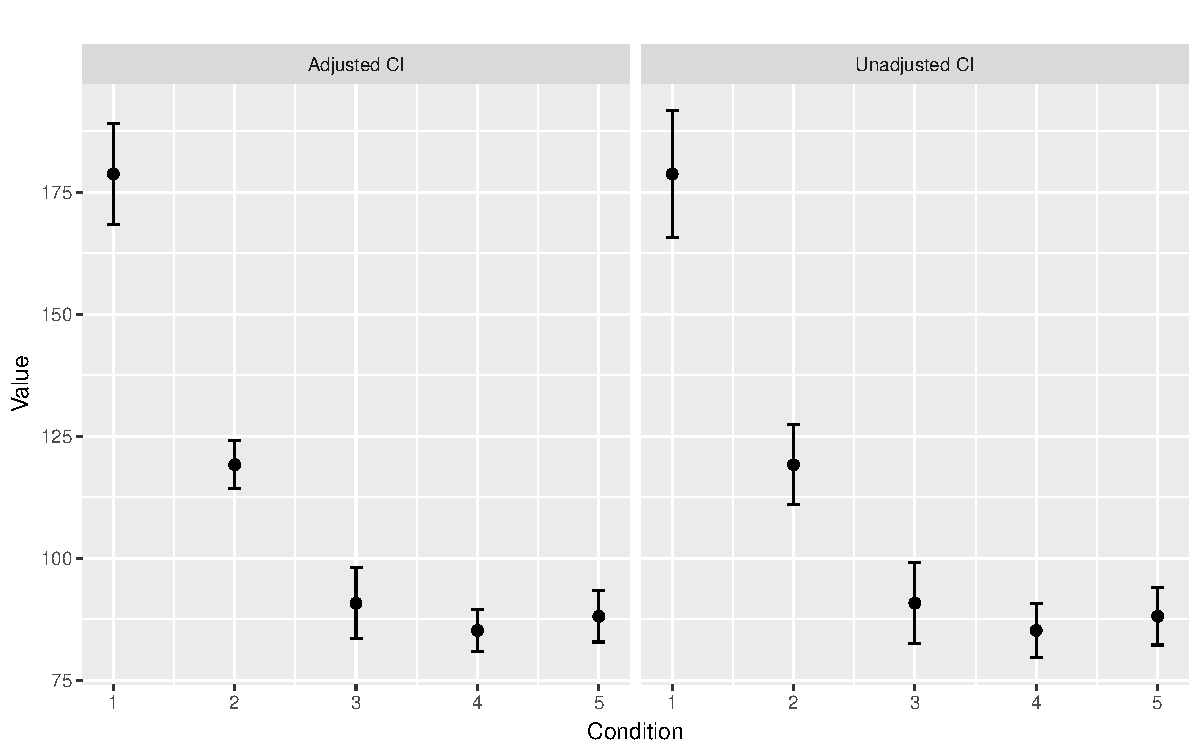
\includegraphics[scale=0.6]{CIs}
				\caption{Adjusted and Unadjusted Confidence Interval}
			\end{center}
		\end{figure}
		
		An important remark is that these confidence intervals should not be used to assess whether the sphericity assumption is violated, which is pointed out by \cite{franz2012standard}. The issues regarding sphericity will be discussed later on in SectionXXX.
		
	\section{Sphericity}
		One of the requirements for a repeated measures ANOVA is known as sphericity. This assumption is met, when the variances of the differences between related combinations of all factor levels are equal. Sphericity is related to homogeneity of variances in an ANOVA without repeated measures. The violation of sphericity causes the test to become too liberal. Therefore, determining whether sphericity has been violated is necessary if the omnibus F-test of a repeated measures ANOVA shall be interpreted. Though violation of sphericity is problematic, it is still possible to conduct and interpret the omnibus F-test if some adjustments for the violation of sphericity are incorporated. This is achieved by estimating the degree to which sphericity has been violated. The corresponding estimator is commonly denoted by epsilon $(\epsilon \in[1,0])$ where a value of 1 indicates that the data is absolute spherical. This measure can then be used as a correction factor to the degrees of freedom of the F-distribution, which leads (in case of $\epsilon<1$) to a decrease in the degrees of freedom and therefore to a more conservative F-test. Of course, it will be only very rarely the case that sphericity is met exactly. Therefore at first, is it is necessary, to test whether it can be assumed that sphericity is theoretically met or not. A popular test to accomplish this is called Mauchly's sphericity test (Mauchly, 1940)cite<---XXX. It tests the $H_0$ that sphericity is met. Therefore a violation of sphericity shall be assumed whenever the Mauchly's sphericity test yields a significant results whereupon the $H_0$ is rejected. Therefore, if a repeated measures ANOVA is appropriate it must be tested whether the assumption of sphericity is met. If it is not met, an appropriate adjustment of the omnibus F-Test has to be performed. This is implemented by the following function:\\
		
		\begin{lstlisting}
# Testing sphericity function
rma_spheri(rma_data, id = 1, append = FALSE)
		\end{lstlisting}
		
		As an input parameter it needs a repeated measures data file which meets the requirements described in sectionXXX. It also contains the $id$ argument. If $append$ is set to \textit{TRUE}, the function chooses the appropriate correction  for the omnibus F-test (\citealp{girden1992anova}) whenever sphericity is violated and appends the thereby adjusted p-value to the ANOVA-table. Obviously, it is nonsensical to test sphericity if there are only two factor levels ($k = 2$). So the function will abort in this case and provide a notification.\\
		
		\begin{lstlisting}
			# Check whether a test for sphericity is needed 
			if (k = 2) {stop("Note that there can't be a violation of sphericity since the factor of the one-way anova has only two factor levels") 
				}
		\end{lstlisting}
		
		To conduct the Mauchly's sphericity test, the first step is to construct a Helmert matrix. The construction of the first row is omitted here since it is not required for further use in this procedure.\\
		
		\begin{lstlisting}
			helmert = function(k, df) { H = matrix(0, k, k) diag(H) = (0:df) * (-((0:df) * ((0:df) + 1))^(-0.5)) for (i in 2:k) { H[i, 1:(i - 1)] = ((i - 1) * (i))^(-0.5) } # H[1,] = 1/sqrt(k) return(H) }
			# The first row of the helmert matrix is not required for further use in this procedure C = helmert(k, df)[-1, ]
		\end{lstlisting}
		
		Thereby, \textit{df} denotes the factor degrees of freedom which equal $k - 1$. Then, the test statistic (Mauchly's W) for the Mauchly's sphericity test is computed by\\
		
		\begin{equation}
		w = \frac{|CVar(Y)C^T|}{(tr(C Var(Y)C^T)k-1)^{k-1}}
		\end{equation}
			
		where \textit{C} is the Helmert matrix and \textit{Var(Y)} is the depended data covariance matrix.\\
		
		\begin{lstlisting}
		# Empirical covariance matrix 
		covariance_matix = cov(dependent_variable)
		w = det(C %*% covariance_matix %*% t(C))/ ((sum(diag(C %*% covariance_matix %*% t(C)))/df)^(df))
		\end{lstlisting}
		
		The transformation 
		
		\begin{equation}
			-(n-1)x(1-\frac{2*(k-1)^2+k+1}{6 x k-1 x n-1}
		\end{equation}
		
		of Mauchly's \textit{W} in $\chi^2$ distributed with
		
		\begin{equation}
			\frac{k*(k-1)}{2}-1
		\end{equation}
		
		
		degrees of freedom. Hence, a p-value for the test can be computed.\\
		
		\begin{lstlisting}
# Computing the degrees of freedom for the chi-square value 
df_w = ((k * df)/2) – 1
# Computing the chi-square value 
f = 1 - ((2 * (df^2) + df + 2)/(6 * df * (n - 1))) 
chi_sq_w = -(n - 1) * f * log(w)
# Computing the corresponding p-value
p_w = 1 - pchisq(chi_sq_w, df_w)
		\end{lstlisting} 
		
		The results of the computational steps described above are summarized in a table, which is later returned by the function \textit{rma_spheri}.
		
		\begin{lstlisting}
			mauchly_table = data.frame(check.names = FALSE, Source = "Factor", `Mauchly's W` = w, `Chi square` = chi_sq_w, df = df_w, p = p_w) rownames(mauchly_table) = NULL
		\end{lstlisting}
		
		The next step is to compute epsilon.
		
		\begin{lstlisting}
			# Lower-Bound correction (Greenhouse & Geisser, 1959) 
			epsilon_lb = 1/df
			# Box correction (Geisser & Greenhouse, 1958) 
			epsilon_gg = (sum(diag(C %*% covariance_matix %*% t(C)))^2)/ (df * sum(diag(t((C %*% covariance_matix %*% t(C))) %*% (C %*% covariance_matix %*% t(C)))))
			# Huynh-Feldt correction (Huynh & Feldt, 1976) 
			epsilon_hf = min((n * df * epsilon_gg - 2)/(df * (n - 1) - (df^2 * epsilon_gg)), 1)
		\end{lstlisting}
		
		There are three commonly used estimators for epsilon (see \cite{rutherford2001introducing}). The Huynh-Feldt epsilon \citep{huynh1976estimation} on the one hand is a fairly liberal estimator, i.e. it tends to underestimate the degree of violation. The Box epsilon \citep{box1954some, geisser1958extension} on the other hand is a more conservative estimator and therefore tends to overestimate the degree of violation. Lastly, the Greenhouse-Geisser or lower bound epsilon (Greenhouse and Geisser, 1959) is the most conservative estimation possible under the given conditions, i.e. it assumes the worst-case scenario of violation. Thus it is actually not sensitive for variation in the degree by which sphericity is violated. Each of these can be used as a correction factor to adjust the degrees of freedom and therefore the resulting p-value of the omnibus F-test (note that the empirical F-value stays the same since the correction factors cancel out, but the theoretical F-distribution of the test statistic under $H_0$ changes).
		
		\begin{lstlisting}
			anova_table = rma(rma_data)[[1]]
			corrected_factor_df = anova_table[2, 3] * epsilon_lb corrected_error_df = anova_table[2, 3] * epsilon_lb p_factor_lb = 1 - pf(anova_table[2, 5], corrected_factor_df, corrected_error_df)
			corrected_factor_df = anova_table[2, 3] * epsilon_gg corrected_error_df = anova_table[2, 3] * epsilon_gg p_factor_gg = 1 - pf(anova_table[2, 5], corrected_factor_df, corrected_error_df)
			corrected_factor_df = anova_table[2, 3] * epsilon_hf corrected_error_df = anova_table[2, 3] * epsilon_hf p_factor_hf = 1 - pf(anova_table[2, 5], corrected_factor_df, corrected_error_df)
		\end{lstlisting}
		
		The results of the computational steps described above are summarized in a table, which is later returned by the function \textit{rma_spheri}.
		
		\begin{lstlisting}
			epsilon_table = data.frame(check.names = FALSE, Source = c("Epsilon", "Adjusted p-Value"), `Lower-Bound correction (Greenhouse & Geisser, 1959)` = c(epsilon_lb, p_factor_lb), `Box correction (Geisser & Greenhouse, 1958)` = c(epsilon_gg, p_factor_gg), `Huynh-Feldt correction (Huynh & Feldt, 1976)` = c(epsilon_hf, p_factor_hf)) rownames(epsilon_table) = NULL
		\end{lstlisting}
		
		\cite{greenhouse1959methods} recommended in case of a violation of sphericity (indicated by a significant Mauchly's sphericity test) to use the lower bound correction first. If the results become insignificant, the Box epsilon is used to estimate the degree of violation. If the degree of violation is high (i.e. $\epsilon < 0.75$), the Box correction is preferable. If the degree of violation is low (i.e. $\epsilon < 0.75$), the Huynh-Feldt epsilon shall be used to correct the degrees of freedom \cite{girden1992anova}.
		
		\begin{lstlisting}
			if (p_w < 0.05) { if (p_factor_lb < 0.05) { anova_table[, "Recommended Lower-Bound corrected p-Value (Greenhouse & Geisser, 1959))"] = c(NA, p_factor_lb, NA, NA, NA, NA) } else { if (epsilon_gg < 0.75) { anova_table[, "Recommended Box corrected p-Value (Geisser & Greenhouse, 1958)"] = c(NA, p_factor_gg, NA, NA, NA, NA) } else { anova_table[, "Recommended Huynh-Feldt corrected p-Value (Huynh & Feldt, 1976)"] = c(NA, p_factor_hf, NA, NA, NA, NA) } } }	
		\end{lstlisting}

		The function will eventually return both tables with the results of the Mauchly's sphericity test as well as the correction factors with their associated adjusted p-values. If the function argument \textit{append} is set to \textit{TRUE}, the ANOVA-table with the recommended p-value is provided as well.		
		
		\begin{lstlisting}
			if (append == TRUE) { return(list(mauchly_table = mauchly_table, correction_factors_epsilon_table = epsilon_table, corrected_anova_table = anova_table)) } else { return(list(mauchly_test_table = mauchly_table, correction_factors_epsilon_table = epsilon_table)) }
		\end{lstlisting}
		
		The analysis of the Ringelmann-data reveals that sphericity is violated $(W=X, \chi^2=X, p<X)$???. The recommended correction is adjusting the degrees of freedom with the Box-epsilon $(\epsilon𝐵𝑜𝑥=𝑋)$. The thereby for the violation in sphericity corrected omnibus F-test is still significant $(F(X,X)=X, p<X)$???. It can therefore be assumed, that there is indeed an effect of the group size on the individual work performance.
		
	
	\section{Orthogonal polynomial contrasts}
		After the conduction of a repeated measures ANOVA we obtain an omnibus F-Value and thus a general idea, whether the factor indeed affects the depended variable. However, it remains unclear what this dependency looks like in particular. To evaluate the impact of the different factor levels on the depended variable in further detail, one might conduct post hock t-tests between each pair of factor levels or even test specific a priori hypothesis by the implementation of complex contrast analyses (see e.g. Howell, 2010; Steavens, 2009). Since the factor levels of a repeated measures ANOVA most commonly possess an interval scale of measurement (or are at least believed to be approximately equidistant ordinal scaled), there is an additional method witch should be considered. This method is known as orthogonal polynomial contrasts or trend analysis. As the name implies, this method detects orthogonal polynomial trend components in the Effects of the factor. If there are k factor levels it decomposes the omnibus factor effect into a full set of $k - 1$ orthogonal contrasts. These contrast all detect a specific polynomial trend of all orders from 1 to $k - 1$ and test if these trends contribute significantly to the overall effect of the factor. This allows testing specific hypothesis regarding separate trends in the depended variable due to manipulations of the factor level.	
		
		\begin{lstlisting}
			rma_opc(rma_data, id = 1, maxpoly = NA, print_plot = TRUE)
		\end{lstlisting}
		
		The above function conducts this type of analysis. As input parameter it needs a repeated measures data file which meets the above described requirements. It also contains the $id = 1$ and $print_plot = TRUE$ Arguments. Since at is always possible to describe the data perfect with a polynom of the order $k - 1$ and hence this is the maximal order of a polynomial trend used for this analysis we define the maxpoly variable. Certainly it is conceivable that not all $k - 1$ orthogonal polynomial trends are of interest, so the function contains the additional argument $maxpoly = NA$. If a Value smaller than $k - 1$ is inserted the function only computes and tests the contrasts up to the polynomial trend of the same order.\\
		
		
		\begin{lstlisting}
		# maximal polynomial degree for orthogonal polynomials if((maxpoly > k - 1) | (is.na(maxpoly))){ maxpoly = k - 1}
		\end{lstlisting}
		
		At first it is necessary to calculate for each of the requested orthogonal trend components a so called linear contrast. A linear contrast is basically the sum of the weighted dependent variable values of each individual factor level. To obtain linear contrasts which represent all orthogonal components of $k - 1$ possible polynomial trends, the weights are generated by using contr.poly().\\
		
		\begin{lstlisting}
		# Defining Contrast weights for orthogonal polynomial contrasts contrast_weights = (t(contr.poly(k)))[1:maxpoly, ]
		\end{lstlisting}
		
		It should be noted, that it needs maxpoly times k contrast weights in total for this type of analysis. In the next step the weighting factors are applied and the linear contrasts for each specific trend are computed individually for each subject
		
		\begin{equation}
		L_S = \sum_{i=1}^{k}c_iY_{is}.
		\end{equation}
		
		\vspace{8 mm}
		
		\begin{lstlisting}
		# Applying formula for linear contrasts 
		weighted_dependend_variables = dependent_variable[rep(1:n, each = maxpoly), ] * (contrast_weights)[rep(1:maxpoly, n), ] linear_subject_contrasts = matrix(rowSums(weighted_dependend_variables), byrow = TRUE, ncol = maxpoly)
		\end{lstlisting}
		
		Following this step there are linear contrasts for each individual entity in the study, so it is necessary to construct an aggregated score to draw further conclusions. This is accomplished by taking the mean of al linear contrasts for one specific trend component to obtain the \textit{contrast\_estimator}\\
		
		\begin{equation}
		\bar{L} = \sum_{i=1}^{n}L_k.
		\end{equation}
		
		\vspace{8 mm}
		
		\begin{lstlisting}
		# Computing contrast estimators for each orthogonal polynomial contrast as well as standard errors for thees estimators
		 contrast_estimator = colMeans(linear_subject_contrasts) contrast_se = sqrt(apply(linear_subject_contrasts,2,var)) / sqrt(n)
		\end{lstlisting}
		
		The standard error of this contrast estimator \textit{contrast\_se} is computed as well for inference reasons. This allows to test whether this contrast score deviates from 0 significantly, which is accomplished via a t-test.\\
		
		\begin{lstlisting}
		# Computing t-values for each contrast contrast_t_values = contrast_estimator / contrast_se #contrast_F_values = contrast_t_values^2
		
		# Computing the corresponding p-values contrast_p_values = 1 - pt(abs(contrast_t_values), n-1)
		\end{lstlisting}
		
		If the individual trend components contribute significantly to the factor effect, it might be of interests how much a certain trend contributed to the effect of the factor. Therefore the sum of squares component which is explained by the factor is decomposed into maxpoly trend component sums of squares by computing the individual trend sum of squares\\
		
	
		\begin{equation}
			SS_L = \frac{n*\bar{L}^2}{\sum_{i=1}^{c_i^2}}
		\end{equation}
		
		\vspace{8 mm}
		
		This is possible due to the fact, that the contrasts are orthogonal to each other, so they do not have redundant information. The proportion of a specific trend sum of square to the factor sum of square marks the percentage in contribution of this particular trend component to the whole factor effect\\
		
		\begin{equation}
			\sum_{j=1}^{k-1}SS_{L(orth.)_j} = SS_{Factor}
		\end{equation}
					
		\vspace{8 mm}
		
		\begin{lstlisting}
			# Computing sums of squares for each contrast 
			contrast_ss = n * contrast_estimator^2 / rowSums(contrast_weights^2)
			
			# Computing amount of the variance in the variable explained by the factor # which in turn can be explained by a cerain orthogonal polynomial trend (ss_trend / ss_factor) 
			proportional_trend_contribution = contrast_ss / rep(sum(rep((Flm - Gm)^2, each = n)), maxpoly)
		\end{lstlisting}
		
		The results of the computational steps described above are summarized in a table, which is later returned by the function.
		
		\begin{lstlisting}
			# define source variable 
			source = rownames(contrast_weights) contrast_table = data.frame(check.names = FALSE, "Source" = source, "Sum of squares" = contrast_ss, "Proportional contribution to the factor effect" = proportional_trend_contribution, "Contrast estimator" = contrast_estimator, "Standard error" = contrast_se, "Degrees of freedom" = rep((n - 1), maxpoly), "t-value" = contrast_t_values, "p-value" = contrast_p_values) rownames(contrast_table) = NULL
		\end{lstlisting}
			
		To display the polynomial trends in the data, polynomial regressions were used. The results actually do not represent orthogonal trends but rather each trend line of a certain polynomial degree also includes all lower order polynomial trend contributions.\\
		
		To store the orthogonal polynomial regression coefficients (OPRC) an empty matrix is set up with k rows and the number of columns equal to the highest order polynomial, previously specified as maxpoly.
		
		\begin{lstlisting}
			poly_coef = data.frame(matrix(0, ncol = maxpoly, nrow = k))	
		\end{lstlisting}
		
		The choice of these dimensions becomes clear when the following code is regarded:
		
		\begin{lstlisting}
			The choice of these dimensions becomes clear when the following code is regarded:
			for (i in 1:maxpoly) {
			pfv = paste("poly_fit_", i, sep = "")
			poly = assign(pfv, lm(rma_data_long$value ~ poly(rma_data_long$condition, degree = i, raw = TRUE)))
			poly_coef[, i][1:(i + 1)] = poly$coef
			}	
		\end{lstlisting}
		
		
		In each cycle of the for loop, that runs from 1 to the maximal polynomial order(maxpoly), the following steps are executed:
		First, orthogonal polynomial regressions are estimated for the observed values (pulled weights) in long format suing the poly() function within lm(). The degree of the highest polynomial is specified by the index i. The model always contains an intercept as well as coefficients for the data to the i-th polynomial. The result, which is an object of type lm, is stored in an object called poly which is overwritten in each cycle.
		In the second step, the coefficients are extracted from poly and stored in the previously prepared matrix (poly\_coef) such that the coefficients are assigned to the i-th column. The subsetting is cruicial here to ensure that the dimensions in the assignment coincide. For example, in the second cycle, the second column of the data frame is chosen. This column is then filled with the intercept coefficient, the first order polynomial coefficient and the second order polynomial coefficient. Since in this cycle there is no higher order, the last element in the data frame remains equal to zero. The resulting data frame looks as follows:
		
		\begin{center}
			\begin{tabular}{ l | c | r }
				19.668 & 4.713  & -60.057 \\
				-4.651  & 10.305  & 113.320\\
				0.000 & -2.991  & -49.255 \\
				0.000 & 0.000  &  6.169 \\
			\end{tabular}
		\end{center}
		Here, one can see that with each cycle of the loop the number of nonzero coefficients increases by one. So the first row stores the coefficients for the intercept, the second row the coefficients for the first order coefficient. The last row always contains the highest order coefficient (here: 3). The columns represent the resulting regression equations and can be seen as follows:\\
		
		\begin{equation}
		C1: b0 + b1X
		C2: b0 + b1X + b2X^2
		C3: b0 + b1X + b2X^2 + b3X^3
		\end{equation}
		
		First, a vector x is defined as a sequence from one to k, the number of factor levels in steps of k/1000. Next, the outer() function is used to create a matrix that takes x to the power of 0 to maxpoly. The result is stored in the object poly\_values.\\
		
		\begin{lstlisting}
			 x = seq(1, k, length.out = 1000)
			 poly_values = outer(x, 0:(k - 1), `^`)
		\end{lstlisting}
		
		The first six rows of the resulting matrix look as following:\\
		
		
		table\\
		
		
		One can see that the first column contains the values for the intercept, just like in a regular linear regression setup. These values are created for the polynomial regression curves that are about to be plotted. Next, a data frame is created containing the vector x and the matrix product of the data matrix poly\_values and the regression coefficients.\\
		
		\begin{lstlisting}
			poly_curve_data = data.frame(x, poly_values %*% poly_coef)
		\end{lstlisting}
		
		The first six rows of the resulting matrix look as following:
		
		Table\\
		
		The columns X1, X2 and X3 contain the estimated y-values from the regression equations stated in XXX for the corresponding x value in the column x.
		The final step is to transform the data to long format which makes plotting with ggplot2 more convenient.\\
		
		\begin{lstlisting}
			poly_curve_data = gather(poly_curve_data, line, y, -x)
		\end{lstlisting}
		
		The resulting data frame is now in long format:\\
		
		Table\\
		
		The final plot is created using \textit{ggplot2} \citep*{wickham2016ggplot2}.
		
		\begin{lstlisting}
			poly_plot = ggplot(data = rma_data_long, aes(x = condition, y = value)) + geom_point() + labs(col = "Order of \npolynomial", x = "Condition", y = "Value", title = "Orthogonal polynomial contrasts") + 
			geom_path(data = poly_curve_data, aes(x, y, color = curve), lwd = 1.2) + scale_color_discrete(labels = as.character(1:(maxpoly))) +
			theme_bw() + theme(panel.grid.major = element_blank(), panel.grid.minor = element_blank(), legend.key = element_rect(colour = "black"), plot.title = element_text(face="bold", hjust = .5))
		\end{lstlisting}
		
		A detailed resource for the use of ggplot2 is provided by \cite{wickham2016ggplot2}. Here, it is worth noticing that the code makes use of ggplot2's ability to plot data from multiple data frames in one plot. On the x-axis there are the factor levels, i.e. the groups from one to four. The y-axis displays the observed values, in this case the individually pulled weight. The data frame rma\_data\_long is used to plot the observed values of the subjects at the different factor levels. The regression curves are plotted using the geom\_path() layer function. The curves are fitted smoothly through the 1000 x-values between 1 and 4 for each regression equation. Here, it is worth noticing that if the number of values for the regression curves is chosen too small, the curves might become wiggly. The color is mapped to the (categorical) curve variable such that each regression curve has a different color. Specifying the color argument withing the aes() function also initializes a legend. The other arguments are used to format the plot.
		
		
		\begin{lstlisting}
			if (print_plot == TRUE){ print(poly_plot)} return(list(contrast_table = contrast_table, poly_plot = poly_plot))
		\end{lstlisting}	
		
		The analysis of the Ringelmann-data reveals a strong and significant linear $(𝑆𝑆𝑙𝑖𝑛.=𝑋, 𝑡(1)=𝑋, 𝑝 <𝑋)$ as well as a quadratic trend $(𝑆𝑆𝑞𝑢𝑎.=𝑋, 𝑡(1)=𝑋, 𝑝 <𝑋)$. In combination with the assessment of the graphical representation of these trend components one shall deduct that the individual work performance is decreasing if the group size increases. In addition is the rate of decrease decreasing as well as the group size increases. This relation between group size and individual work performance was also already pointed out by \cite{kravitz1986ringelmann}.
		
		\section{R Packages}
		Packages in R are bundles of code, documentation, data and tests \citep{wickham2015r}. They make up a fundamental part of the R language since they allow to share code with other R users. In other programming languages these units are often referred to as libraries. The constantly growing amount of R packages is one characteristic of R as an open source software \citep{chambers2008software}. Packages can be downloaded from CRAN (https://cran.r-project.org/) which provides the official repository for R packages as well as from GitHub via the devtools package \cite. Currently (January 26th, 2017), there are 9988 packages available on the CRAN website.\\
		
		There are a few noticeable aspects why packages form such a fundamental basis of R. First, they allow to share code with others which enables a consistently growing range of functionalities in R. Moreover, when loading a package, all functions of that package are automatically loaded into the namespace. This is very time-saving especially when a package is frequently used as opposed to sourcing scripts with the required functions. Dependencies, other packages that the loaded package requires, are automatically loaded or even installed if necessary. And finally, the documentation of functions in a package allows the creator of the package as well as other users to understand the way a function works.\\
		
		A personal motivation to create a package for repeated measures ANOVA was there were functionalities, like the adjusted confidence intervals, that we needed for a research project which had not been implemented in R, or at least not conveniently bundled in a single package. The MAGA package is an attempt to fill this void and provide the functionalities for other R users and researchers that use repeated measures ANOVA.\\
		
		The Quantlet structure of the code made it easy to choose the functionalities that were turned into a function in the package. For creating the package, devtools \citep{wickham2015devtools} and roxygen2 \citep{wickham2013roxygen2} were used. While devtools automates different tasks of package development, roxygen2 can be used to write package documentation directly into the R scripts of the functions which is then compiled to Rd format \citep{wickham2013roxygen2}. Since the MAGA package has not been published on CRAN yet (January, 26th 2017), devtools::install.github() may be used to install the package from its GitHub repository.\\
		
		When writing the package, we carefully chose function names that indicate what the function does for a convenient use of the package. Another topic which is especially relevant when writing a package is error handling. This is crucial to ensure that the functions are robust against violation of the requirements of the function arguments. In each of the functions of the package, a sequence of if-statements was implemented to check if the requirements of the function input were met. When considering error handling in package creation it is important to differentiate between the functions stop() and warning(). Both return a message to the user but only stop() interrupts the code. So whenever we checked for requirements that were essential for the function to work we chose stop(). Additionally, the function documentation specifies the data type of each argument (see section about function documentation).
		The following code displays the if-statements that were used to check whether the input data meets the requirements:\\
		
		\begin{lstlisting}
			# id must either be an integer specifying the column position of the independent variable
			if (id %in% 1:ncol(rma_data) == FALSE || length(id) != 1) {
			stop("id must be an integer specifying the column position of the independent variable")
			}
		\end{lstlisting}
		
		This part of the code ensures that the id variable is specified via a single integer which specifies the column position of the ID variable. This variable is an index variable which numerates the subjects. If the variable is not an integer between 1 and the number of columns of the input data an error message is returned.\\
		
		\begin{lstlisting}
		# all variables must be numeric
		if (all(sapply(rma_data, is.numeric)) == FALSE | any(sapply(rma_data, is.factor))) {
		stop("All variables in rma_data must be numeric")
		}
		\end{lstlisting}
		
		This if-statement controls for the right data type. All variables of the data must be numeric. Since R considers factor variables numeric, the code after the logical OR ensures that the function is also interrupted when one or more variables are factors. Again, an error message is returned in that case to inform the user about the requirements.ẞẞ
		
		\begin{lstlisting}
			# n > k (i.e. more entities than factor levels)
			if (n <= k) {
			stop("Number of entities must exceed number of factor levels")
			}
		\end{lstlisting}
		
		Moreover, for ANOVA methods to work, the number of subjects needs to exceed the number of factor levels. This means that the number of rows (automatically defined as n by the function) has to be strictly larger than k (the number of columns minus one for the index variable).\\
		
		\begin{lstlisting}
		    # k >= 2 (i.e. at least two or more factor levels)
		    if (k < 2) {
		    stop("At least two factor factor levels required")
		    }  
		\end{lstlisting}
		
		Finally, the data needs to have at least two factor levels, since otherwise no ANOVA model can be estimated. This is controlled by the last of the if-statements.
		A particular case where the warning() function was used is described in section XXX.
		Function documentation can be demonstrated on one particular function since the necessary steps apply to all other functions as well. For demonstration purposes, the function ow\_rma\_opc was chosen. The following code is compiled by roxygen2 to an Rd file which contains the information that are displayed when the help page in R is called, for example via the command ?ow\_rma\_opc.\\
		
		\begin{lstlisting}
		Each line in the documentation needs to start with #'.
		The first line is the heading of the help page and summarizes briefly what the function does.
		#' Estimate and plot orthogonal polynomial trends
		#'
		
		The next line is displayed by roxygen2 via the heading Description and features short yet precise information about the function.
		#' Compute orthogonal polynomial contrasts and plot orthogonal polynomial regression curves for a repeated measures ANOVA.
		#'
		
		The next section Usage is automatically created by roxygen2. It demonstrates how to call the function.
		
		Via @param the function parameters are listed under the heading Arguments. Here, it is important to inform the user about the required data types, e.g. numeric vector or data.frame. Moreover, default values, if existing, are documented.
		#' @param ow_rma_data An object of type data.frame. Each row should represent one subject and each column one variable.
		#' @param id An integer specifying the column position of the subject ID. Default is 1. Set to "none" if the data does not contain an ID variable.
		#' @param maxpoly Integer. Specifies the highest order polynomial for the contrast analysis. Truncated to number of factor levels (k) -1 if larger. Default is NA which will be set to k-1 within the function.
		#'
		
		In the next step, the object(s) that the function returns need to be specified. This is achieved via @return and summarized under the section label Value. Here,  the function returns a list. In the next lines \item is used to describe the objects in particular. The list stores a data frame containing the results from the polynomial contrast analysis and the ggplot object that displays the orthogonal polynomial regression curves.
		#' @return Returns an object of type list.
		#' \item{contrast_table}{An object of type data.frame containing the contribution of the polynomial trends to the total factor effect and their respective significance levels}
		#' \item{poly_plot}{A ggplot object. Displays the orthogonal polynomial regression curves.}
		
		The last sections contain the authors’ names, notes, literature and examples if provided.
		#' @author Joachim Munch, Frederik Schreck, Quang Nguyen Duc, Constantin Meyer-Grant, Nikolas Hoeft
		#' @note LITERATURE
		#' @examples
		#'
		
		Finally @rdname specifies where the documentation is stored, here for the function ow_rma_opc, and @export is especially important to ensure that the function is added to the namespace file.
		#' @rdname ow_rma_opc
		#' @export
		\end{lstlisting}
		
		A final word needs to be said about the description file. A template for this is automatically created when building a new package in RStudio. Basically, this file contains some meta data about the package like a description, which does not require further elaboration. One important aspect though is the use of dependencies. These are other packages that are required to run the functions in the new package. In the section Imports the names of the required packages are specified. When the MAGA package is installed, R automatically ensures that the dependencies (here: dplyr, ggplot2 and tidyverse) are installed as well. Moreover, they are also loaded whenever MAGA is loaded via the library() command.\\
		\\
		Package: MAGA
		Type: Package
		Title: A package to make ANOVA great again!
		Version: 0.1.0
		Author: Joachim Munch, Frederik Schreck, Quang Nguyen Duc, Constantin Meyer-Grant, Nikolas Hoeft
		Maintainer: Nikolas Hoeft <nikolas.hoeft@hu-berlin.de>
		Description: A package for repeated measures ANOVA models. 
		Allows to simulate data, compute ANOVA and RM ANOVA 
		models, investigate error term reduction due to model selection, 
		compute and display adjusted confidence intervals. 
		Furthermore it enables to conduct Mauchly's test for 
		sphericity and it provides various correction factors to 
		adjust p-values in the presence of sphericity. The package 
		also supplies a function to fit orthogonal polynomial 
		contrasts and to plot orthogonal polynomial regression curves.
		Imports:
		dplyr,
		ggplot2,
		tidyverse
		License: 
		Encoding: UTF-8
		LazyData: true
		RoxygenNote: 5.0.1
		
		
		Of course there are many other possible steps for package development. The ones described above however are the most important and basic ones and were therefore chosen for this report.
		
		
		
		
		
	

 
 % Damit der Anhang nicht im Inhaltsverzeichnis auftaucht.
	\section*{Appendix}
	\newpage
 \bibliography{lit}
 \bibliographystyle{dcu}
 \addcontentsline{toc}{section}{Literature}

	



\end{document}
